% Informe de la Pràctica 2, part 1 (classificació d'intencions). Compila amb pdflatex, dues passades, des
% d'aquesta carpeta, amb figures_practica_2_1/ al costat. Mateix format que l'informe de la part 2.
\documentclass[11pt,a4paper]{article}

\usepackage[utf8]{inputenc}
\usepackage[T1]{fontenc}
\usepackage[catalan]{babel}
\usepackage{lmodern}
\usepackage[a4paper,margin=2cm]{geometry}
\usepackage{graphicx}
\usepackage{booktabs}
\usepackage{array}
\usepackage{amsmath}
\usepackage[round,authoryear]{natbib}
\usepackage[hidelinks]{hyperref}
% microtype i caption milloren la tipografia però no són imprescindibles: si la instal·lació no els té
% (TinyTeX mínim), el document compila igualment.
\IfFileExists{microtype.sty}{\usepackage{microtype}}{}
\IfFileExists{caption.sty}{\usepackage{caption}\captionsetup{font=small,labelfont=bf}}{}

\graphicspath{{figures_practica_2_1/}}
\setlength{\parskip}{0.3em}
\setlength{\bibsep}{2pt}

% Noms d'intenció en tipus fix; detokenize permet escriure guions baixos i signes + tal qual.
\newcommand{\intent}[1]{\texttt{\detokenize{#1}}}

\title{Pràctica 2, part 1: classificació d'intencions a ATIS}
\author{Laia Beyloc Guzmán \and Ilyas Ouacham Rhailane}
\date{Tractament de la Veu i el Diàleg\\[4pt]\today}

\begin{document}
\maketitle

\section{Introducció}
\label{sec:intro}

Abans de poder respondre, un sistema conversacional ha de saber què li demana l'usuari: si busca un vol, el preu
d'un bitllet o el tipus d'avió que fa una ruta. En aquesta part de la pràctica classifiquem cada consulta en una
d'aquestes intencions. La dificultat és que dues frases poden compartir gairebé totes les paraules i demanar
coses diferents, com ``flights from boston to denver'' i ``fares from boston to denver'', i per això hem comparat
models que només agreguen les paraules amb models que tenen en compte patrons locals o l'ordre de la seqüència.

Als exercicis 1-4 hem completat la tokenització, el padding, la codificació d'etiquetes i el model inicial. A
l'exercici 5 hem estudiat el vocabulari, la normalització del text, la mida dels embeddings, xarxes CNN, LSTM i GRU,
la bidireccionalitat, l'atenció, el dropout i la ponderació de classes, i hi hem afegit una comparació petita de
self-attention amb i sense informació posicional.

\section{Experiments i resultats}
\label{sec:experiments}

% ---------------------------------------------------------------------------------------------------------
\subsection{Dades i preprocessament (exercicis 1-3)}
\label{sec:dades}

Treballem amb ATIS, el corpus de consultes sobre vols de la pràctica, amb oracions en anglès. Cada cadena
d'etiqueta és una classe, incloses les compostes amb \(+\) (per exemple \intent{flight+airfare}), és a dir, no
hem plantejat el problema com a multietiqueta. Les primeres 4.078 files del CSV d'entrenament són train i les 900
últimes, validació, tal com indica l'enunciat (taula~\ref{tab:particions}).

\begin{table}[ht]
\centering\small
\caption{Particions utilitzades. Les classes es compten després del filtratge.}
\label{tab:particions}
\begin{tabular}{lrrr}
\toprule
Partició & Exemples originals & Exemples utilitzats & Classes presents\\
\midrule
Train & 4.078 & 4.078 & 22\\
Validació & 900 & 900 & 17\\
Test & 893 & 888 & 16\\
\bottomrule
\end{tabular}
\end{table}

De test hem tret cinc exemples perquè les seves etiquetes no surten mai a train: dos de \intent{day_name} i un
de \intent{airfare+flight}, \intent{flight+airline} i \intent{flight_no+airline}. A validació no n'hi ha cap. Per
tant, el que mesurem és la classificació entre intencions conegudes, no la detecció d'intencions noves.

Tokenitzem per paraules amb PAD=0 i UNK=1, de manera que les paraules conegudes comencen a l'índex 2, i el límit
de vocabulari compta els dos índexs reservats (amb 500, el model coneix 498 paraules). El codi original
eliminava les paraules desconegudes; ara les substituïm per UNK i així no es perd la seva posició dins de la
frase. Tant el vocabulari com la longitud màxima (48 tokens) s'aprenen només amb train, i el padding va al final.

Hi ha dos aspectes de les dades que condicionen tota la interpretació. El primer és el desequilibri:
\intent{flight} té 3.023 dels 4.078 exemples de train (74,13\%), mentre que quatre classes només en tenen un i
dues, dos. El segon és que hi ha textos repetits entre particions. Les files són diferents, però 93 textos de train
tornen a aparèixer a validació (en 104 files) i 10 a test, cosa que pot fer els resultats una mica optimistes.

% ---------------------------------------------------------------------------------------------------------
\subsection{Model inicial (exercici 4)}
\label{sec:inicial}

El model inicial converteix cada paraula en un embedding de 64 dimensions, en fa un global max pooling i passa el
resultat per una capa lineal de 64 unitats amb ReLU i una capa final de 22 sortides. Al pooling ignorem les
posicions de padding, ja que altrament el vector de PAD, que és de zeros, podria substituir activacions negatives
en el màxim. Com a loss fem servir \texttt{CrossEntropyLoss}, que rep els índexs de classe i ja inclou el softmax
\citep{ce}.

L'hem entrenat amb Adam (learning rate 0,001), batch 32, fins a 30 èpoques i \emph{early stopping} amb paciència 3.
A l'execució guardada, el model s'atura a l'època 25 i recupera els pesos de menor loss de validació (0,3036), amb
una accuracy de validació del 92,78\% (835/900). Aquest entrenament no fixa la llavor, i per això el resultat
canvia una mica d'una execució a una altra; a l'exercici 5 sí que les fixem.

% ---------------------------------------------------------------------------------------------------------
\subsection{Metodologia de l'exercici 5}
\label{sec:metodologia}

Tots els experiments de l'exercici 5 comparteixen el mateix protocol (taula~\ref{tab:protocol}). Els pesos
s'aprenen només amb train, la validació serveix per aturar l'entrenament i per triar configuracions, i el test
l'hem fet servir una sola vegada, amb el model final. Quan entrenem amb pesos de classe, el checkpoint es tria
igualment amb la loss de validació sense pesos, perquè el criteri sigui el mateix en tots els casos.

\begin{table}[ht]
\centering\small
\caption{Protocol comú de l'exercici 5.}
\label{tab:protocol}
\begin{tabular}{ll}
\toprule
Element & Configuració\\
\midrule
Optimitzador / learning rate & Adam / 0,001\\
Batch / màxim d'èpoques & 32 / 25\\
Early stopping & Paciència 4, sobre la loss de validació sense pesos\\
Llavor dels contrastos & 42\\
Llavors dels finalistes & 42, 123 i 2026\\
Checkpoint & Pesos de loss de validació mínima\\
Criteri de selecció & Accuracy; en cas d'empat, macro-F1 i després loss\\
\bottomrule
\end{tabular}
\end{table}

A més de l'accuracy, calculem la macro-F1 sobre les 22 classes de train,
\[
  F_{1,\mathrm{macro}}=\frac{1}{22}\sum_{c=1}^{22}\frac{2\,TP_c}{2\,TP_c+FP_c+FN_c},
\]
on una classe sense cap predicció ni cap exemple compta com a zero \citep{f1}. Com que validació té 17 classes i
test 16, la macro-F1 inclou zeros de classes que no hi apareixen. Per això és molt més baixa que l'accuracy i s'ha
de llegir juntament amb els suports.

En total hem fet 32 entrenaments: 30 dels apartats principals i 2 de la comparació de self-attention. Dues
configuracions més (vocabulari 2000 i minúscules desactivades) generen exactament els mateixos tensors que altres
ja entrenades, i en reutilitzem el resultat. El notebook s'executa sencer amb \emph{Restart \& Run All} en CPU.
A cada contrast canviem un sol factor amb la llavor 42, i totes les accuracies que donem fins a
l'apartat~\ref{sec:global} són de validació.

% ---------------------------------------------------------------------------------------------------------
\subsection{Preprocessament i vocabulari}
\label{sec:vocab}

Hem provat límits de 250, 500, 1.000 i 2.000 identificadors amb el model inicial (embedding 64, sense dropout) i,
amb vocabulari 500, l'efecte de passar a minúscules i del stemming de Snowball (taula~\ref{tab:vocab}).

\begin{table}[ht]
\centering\small
\caption{Vocabulari i normalització amb el model inicial.}
\label{tab:vocab}
\begin{tabular}{lrr}
\toprule
Configuració & Accuracy (\%) & Macro-F1\\
\midrule
Vocabulari 250 & 92,56 & 0,4733 \\
Vocabulari 500 (referència) & 93,56 & 0,4565 \\
Vocabulari 1.000 & 93,89 & 0,4255 \\
Vocabulari 2.000 & 93,89 & 0,4255 \\
Vocabulari 500 + stemming & 92,89 & 0,4113 \\
\bottomrule
\end{tabular}
\end{table}

Ampliar el vocabulari de 250 a 1.000 paraules millora l'accuracy 1,33 punts, però la macro-F1 baixa de 0,4733 a
0,4255. El vocabulari gran beneficia les classes freqüents, i amb només 900 frases de validació les classes rares
pesen molt en la macro-F1. Amb 1.000 ja cobrim les 830 paraules diferents de train, i per això 2.000 dona
exactament el mateix resultat. Hem triat 1.000 per accuracy, que és el criteri del protocol.

Passar a minúscules no canvia res, perquè els textos ja hi estan, i el stemming empitjora tant l'accuracy com la
macro-F1. Tampoc no hem tret stopwords, perquè paraules com \emph{from}, \emph{to} o \emph{not} són necessàries
per entendre bé la consulta.

% ---------------------------------------------------------------------------------------------------------
\subsection{Dimensió dels embeddings}
\label{sec:emb}

\begin{table}[ht]
\centering\small
\caption{Mida de l'embedding (vocabulari 500, capa oculta 64).}
\label{tab:emb}
\begin{tabular}{rrrr}
\toprule
Dimensió & Accuracy (\%) & Macro-F1 & Paràmetres\\
\midrule
32 & 90,67 & 0,3668 & 19.542 \\
64 & 93,56 & 0,4565 & 37.590 \\
128 & 93,67 & 0,4797 & 73.686 \\
\bottomrule
\end{tabular}
\end{table}

De 32 a 64 dimensions la millora és clara, de gairebé tres punts (taula~\ref{tab:emb}). De 64 a 128, en canvi,
l'accuracy només guanya un encert de 900 i la macro-F1 puja 0,02, mentre que els paràmetres gairebé es dupliquen.
Com que un guany en vocabulari i un altre en embedding no tenen per què sumar-se, hem entrenat també la combinació
de vocabulari 1.000 i embedding 128, que arriba al 94,11\% amb macro-F1 0,4500. És la representació que hem fet
servir en la resta d'experiments.

% ---------------------------------------------------------------------------------------------------------
\subsection{Xarxes convolucionals}
\label{sec:cnn}

Hem provat una convolució de 64 filtres amb kernels de 2, 3 i 5 i max pooling, i després, amb el millor kernel,
hem comparat el max pooling amb l'average pooling i hem afegit una segona convolució (taula~\ref{tab:cnn}).

\begin{table}[ht]
\centering\small
\caption{CNN amb vocabulari 1.000 i embedding 128.}
\label{tab:cnn}
\begin{tabular}{lrrr}
\toprule
Configuració & Accuracy (\%) & Macro-F1 & Paràmetres\\
\midrule
Una capa, kernel 2, max & 95,56 & 0,5501 & 124.374 \\
Una capa, kernel 3, max & 94,89 & 0,5096 & 132.566 \\
Una capa, kernel 5, max & 92,00 & 0,4534 & 148.950 \\
Una capa, kernel 2, average & 95,78 & 0,5668 & 124.374 \\
Dues capes, kernel 2, max & 95,78 & 0,5676 & 132.630 \\
\bottomrule
\end{tabular}
\end{table}

Amb kernels de 2 i 3, la CNN supera la millor configuració del model inicial (94,11\%), però com més gran és el
kernel, pitjor va, i amb 5 ja queda per sota. Una part de l'explicació és que 33 frases de validació tenen menys
de cinc tokens i, amb un kernel de 5, no tenen cap finestra completa, de manera que la seva representació queda a
zero. També és possible que, en consultes tan curtes, les parelles de paraules (``what time'', ``how much'') ja
siguin prou informatives.

L'average pooling i les dues convolucions empaten en accuracy (95,78\%). La versió de dues capes té 0,0007 més de
macro-F1 i 8.256 paràmetres més, i l'hem triada pel criteri de desempat, tot i que la diferència és mínima.

% ---------------------------------------------------------------------------------------------------------
\subsection{Xarxes recurrents}
\label{sec:rnn}

Hem comparat LSTM i GRU, unidireccionals i bidireccionals, i també la LSTM amb una atenció escalar que fa una
mitjana ponderada dels estats ocults (no és self-attention). Totes tenen una capa, 128 unitats i cap dropout, i
processen les frases amb \texttt{pack\_padded\_sequence} perquè el padding no modifiqui l'estat
(taula~\ref{tab:rnn}).

\begin{table}[ht]
\centering\small
\caption{Xarxes recurrents amb la mateixa representació i entrenament.}
\label{tab:rnn}
\begin{tabular}{lrrr}
\toprule
Arquitectura & Accuracy (\%) & Macro-F1 & Paràmetres\\
\midrule
LSTM & 96,22 & 0,5455 & 241.430 \\
BiLSTM & 97,00 & 0,6268 & 376.342 \\
GRU & 96,67 & 0,6168 & 208.406 \\
BiGRU & 97,00 & 0,6037 & 310.294 \\
LSTM + atenció & 97,11 & 0,6164 & 241.559 \\
BiLSTM + atenció & 96,78 & 0,6085 & 376.599 \\
\bottomrule
\end{tabular}
\end{table}

Totes les recurrents superen les CNN en accuracy, i totes menys la LSTM simple també en macro-F1. La
bidireccionalitat millora l'accuracy de la LSTM i de la GRU, encara que a la GRU fa baixar la macro-F1. L'atenció
millora la LSTM 0,89 punts amb només 129 paràmetres més, però sobre la BiLSTM empitjora totes dues mètriques. Hem
triat la LSTM amb atenció, la de millor accuracy, i hem comprovat que reduir-ne la capa oculta a 64 unitats
empitjora el resultat (96,33\% i 0,5152), de manera que mantenim les 128.

Cal dir, però, que entre aquestes sis variants les diferències són de com a màxim 8 encerts sobre 900, amb una
sola llavor. El que sí que es pot defensar és que les recurrents superen les CNN i el model inicial; l'ordre entre
elles és menys segur.

% ---------------------------------------------------------------------------------------------------------
\subsection{Self-attention i posicions}
\label{sec:sa}

Fora de la selecció principal, hem comparat un model de self-attention amb quatre capçals, una mitjana de les
posicions i un classificador, amb i sense embeddings posicionals apresos (taula~\ref{tab:sa}). Sense posicions,
el model no té cap manera de saber en quin ordre van les paraules.

\begin{table}[ht]
\centering\small
\caption{Self-attention amb i sense posicions (llavor 42; temps en segons).}
\label{tab:sa}
\begin{tabular}{lrrrr}
\toprule
Variant & Accuracy (\%) & Macro-F1 & Paràmetres & Temps\\
\midrule
Sense posicions & 93,11 & 0,4548 & 175.382 & 7,94 \\
Amb posicions & 94,11 & 0,5065 & 181.526 & 9,01 \\
\bottomrule
\end{tabular}
\end{table}

Les posicions aporten nou encerts més de validació i 0,05 de macro-F1, a canvi de 6.144 paràmetres més. Això
indica que l'ordre ajuda, tot i que amb una sola llavor i sense un control amb el mateix nombre de paràmetres no
podem separar del tot l'efecte de l'ordre del de la capacitat afegida. Aquesta comparació estava pensada des del
principi fora de la selecció del model final, i en tot cas cap de les dues variants arriba a les recurrents.

% ---------------------------------------------------------------------------------------------------------
\subsection{Regularització}
\label{sec:dropout}

Hem provat dropout de 0, 0,2 i 0,4 abans del classificador, en la CNN i en la LSTM amb atenció triades als
apartats anteriors (taula~\ref{tab:dropout}).

\begin{table}[ht]
\centering\small
\caption{Efecte del dropout.}
\label{tab:dropout}
\begin{tabular}{rrrrr}
\toprule
 & \multicolumn{2}{c}{CNN de dues capes} & \multicolumn{2}{c}{LSTM + atenció}\\
Dropout & Accuracy (\%) & Macro-F1 & Accuracy (\%) & Macro-F1\\
\midrule
0 & 95,78 & 0,5676 & 97,11 & 0,6164 \\
0,2 & 95,56 & 0,5385 & 96,78 & 0,5607 \\
0,4 & 95,67 & 0,5289 & 97,11 & 0,6186 \\
\bottomrule
\end{tabular}
\end{table}

\begin{figure}[ht]
\centering
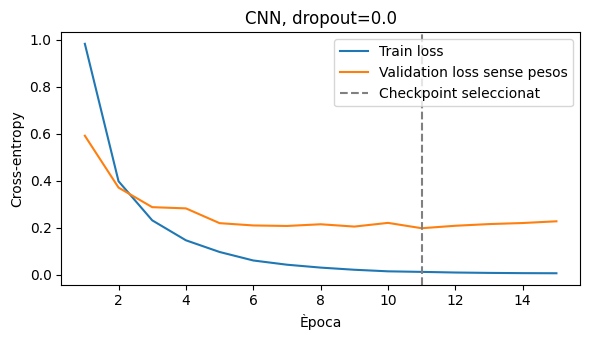
\includegraphics[width=0.62\linewidth]{sobreajustament_cnn}
\caption{CNN sense dropout: la loss de train continua baixant i la de validació puja a partir del checkpoint de
l'època 11.}
\label{fig:cnn}
\end{figure}

A la CNN, el dropout no millora res. La figura~\ref{fig:cnn} mostra que el sobreajust hi és, però l'\emph{early
stopping} ja atura l'entrenament a l'època 11, abans que la loss de validació comenci a pujar. A la LSTM amb
atenció, el dropout de 0,2 empitjora, mentre que el de 0,4 empata en accuracy amb 0,0022 més de macro-F1. Hem
mantingut la CNN sense dropout i la LSTM amb 0,4, sabent que en aquest segon cas la diferència és molt petita.

% ---------------------------------------------------------------------------------------------------------
\subsection{Balanceig de classes}
\label{sec:balanceig}

Com que \intent{flight} representa el 74\% de train, un model pot tenir una accuracy alta i fallar gairebé totes
les classes rares. Per compensar-ho hem ponderat la loss amb pesos calculats a partir de les freqüències de train,
\[
 w_c=\frac{N}{C\,n_c},\qquad N=4.078,\quad C=22,
\]
que donen valors molt extrems per a les classes més petites (taula~\ref{tab:pesos}).

\begin{table}[ht]
\centering\small
\caption{Classe majoritària i les sis classes amb una o dues mostres de train.}
\label{tab:pesos}
\begin{tabular}{lrrr}
\toprule
Classe & Exemples & Freqüència (\%) & Pes\\
\midrule
\intent{flight} & 3.023 & 74,13 & 0,0613 \\
\intent{restriction} & 2 & 0,05 & 92,68 \\
\intent{airline+flight_no} & 2 & 0,05 & 92,68 \\
\intent{aircraft+flight+flight_no} & 1 & 0,02 & 185,36 \\
\intent{airfare+flight_time} & 1 & 0,02 & 185,36 \\
\intent{cheapest} & 1 & 0,02 & 185,36 \\
\intent{ground_service+ground_fare} & 1 & 0,02 & 185,36 \\
\bottomrule
\end{tabular}
\end{table}

Amb aquesta fórmula, un exemple d'una classe amb una sola mostra pesa 3.023 vegades més que un de
\intent{flight}. Els pesos no afegeixen informació nova, i un model que veu un sol exemple d'una classe té molta
facilitat per memoritzar-lo. Amb la LSTM amb atenció i dropout 0,4, els pesos mantenen l'accuracy en el 97,11\% i
pugen la macro-F1 de 0,6186 a 0,6451 (taula~\ref{tab:recall}).

\begin{table}[ht]
\centering\small
\caption{Recall de validació per classe, sense i amb pesos.}
\label{tab:recall}
\begin{tabular}{lrrr}
\toprule
Classe & Suport & Sense pesos & Amb pesos\\
\midrule
\intent{aircraft} & 13 & 0,9231 & 1,0000 \\
\intent{airport} & 6 & 0,6667 & 0,8333 \\
\intent{flight_time} & 8 & 0,8750 & 1,0000 \\
\intent{restriction} & 4 & 0,0000 & 0,2500 \\
\intent{airline} & 32 & 0,8750 & 0,9063 \\
\intent{flight+airfare} & 6 & 0,6667 & 0,8333 \\
\intent{flight} & 643 & 0,9953 & 0,9860 \\
\intent{meal} & 3 & 0,0000 & 0,0000 \\
\bottomrule
\end{tabular}
\end{table}

Cada millora de la taula correspon a un sol exemple encertat de més. A \intent{flight}, en canvi, el model passa de
640 a 634 encerts sobre 643, i les dues coses es compensen en l'accuracy, mentre que \intent{meal} continua sense
cap encert. Hem mantingut el model amb pesos perquè té més macro-F1 amb la mateixa accuracy, però amb guanys d'un
exemple per classe la millora és fràgil, i cinc classes de train ni tan sols tenen exemples a validació.

% ---------------------------------------------------------------------------------------------------------
\subsection{Comparació global i selecció del model}
\label{sec:global}

Per veure si les diferències entre famílies es mantenen amb altres inicialitzacions, hem repetit el millor model
de cada família amb les llavors 42, 123 i 2026 (taula~\ref{tab:finalistes}).

\begin{table}[ht]
\centering\small
\caption{Validació amb tres llavors (mitjana $\pm$ desviació); paràmetres i temps de la llavor 42.}
\label{tab:finalistes}
\begin{tabular}{lrrrr}
\toprule
Finalista & Accuracy (\%) & Macro-F1 & Paràmetres & Temps (s)\\
\midrule
Feedforward & 93,74 $\pm$ 0,46 & 0,4400 $\pm$ 0,0189 & 116.182 & 6,55 \\
CNN, dues convolucions & 96,00 $\pm$ 0,38 & 0,5617 $\pm$ 0,0230 & 132.630 & 9,37 \\
LSTM + atenció, ponderada & 97,30 $\pm$ 0,23 & 0,6531 $\pm$ 0,0209 & 241.559 & 26,90 \\
\bottomrule
\end{tabular}
\end{table}

Les diferències entre famílies són més grans que la variació entre llavors. La recurrent supera la CNN en 1,3
punts d'accuracy i 0,09 de macro-F1, i la CNN supera el feedforward en 2,3 punts. Hem triat la família recurrent,
que és la millor en totes dues mètriques, encara que costa gairebé el doble de paràmetres i el triple de temps
d'entrenament que la CNN.

El model final és, doncs, la LSTM unidireccional amb atenció, vocabulari 1.000 (832 identificadors reals),
embedding i capa oculta de 128, dropout 0,4 i pesos de classe, entrenada amb la llavor 42. Vam fixar aquesta llavor
abans de la comparació, i per això no hem agafat la 123 tot i que dona més accuracy de validació. Els pesos
restaurats són els de l'època 13, amb una loss de validació de 0,1435, una accuracy del 97,11\% i una macro-F1 de
0,6451.

% ---------------------------------------------------------------------------------------------------------
\subsection{Avaluació final sobre test}
\label{sec:test}

Sobre els 888 exemples de test, el model encerta 848 (accuracy del 95,50\%), amb macro-F1 0,5937 i loss 0,2061.
No hem provat cap altre model a test.

\begin{table}[ht]
\centering\small
\caption{Exemples del comportament per classe a test.}
\label{tab:test}
\begin{tabular}{lrrr}
\toprule
Classe & Suport & Encerts & Recall\\
\midrule
\intent{flight} & 632 & 613 & 0,9699 \\
\intent{airfare} & 48 & 48 & 1,0000 \\
\intent{city} & 6 & 1 & 0,1667 \\
\intent{flight+airfare} & 12 & 5 & 0,4167 \\
\intent{meal} & 6 & 3 & 0,5000 \\
\intent{flight_time} & 1 & 1 & 1,0000 \\
\bottomrule
\end{tabular}
\end{table}

L'accuracy de test és 1,6 punts més baixa que la de validació, i el rendiment per classe és molt desigual
(taula~\ref{tab:test}). Les classes freqüents com \intent{airfare} surten gairebé perfectes, però \intent{city}
només encerta un dels sis casos i \intent{flight+airfare}, cinc de dotze. A la matriu de confusió del notebook es
veu que molts d'aquests errors acaben classificats com a \intent{flight}, la classe que domina l'entrenament. La
macro-F1 de test (0,5937) inclou zeros de les sis classes de train que no apareixen a test, i per això no s'ha de
comparar directament amb l'accuracy.

\section{Conclusions}
\label{sec:conclusions}

Les arquitectures que tenen en compte l'ordre de les paraules han estat millors que el model inicial, que només
agrega els embeddings. Amb tres llavors, la LSTM amb atenció arriba al 97,30\% de validació, la CNN al 96,00\% i el
feedforward al 93,74\%, unes diferències més grans que la variació entre llavors. Dins de cada família, en canvi,
moltes diferències són de pocs encerts amb una sola llavor, i no les hem tractat com a concloents.

Ampliar el vocabulari i els embeddings millora l'accuracy, però no sempre la macro-F1, perquè les millores es
concentren en les classes freqüents. Ni el stemming ni el dropout han ajudat, i a la CNN l'\emph{early stopping} ja
controla el sobreajust. Els pesos de classe han pujat la macro-F1 0,026 sense perdre accuracy, encara que a costa
d'algun error més a \intent{flight} i amb millores d'un sol exemple a les classes rares.

El model final obté un 95,50\% d'accuracy a test, amb un rendiment molt desigual entre classes, i hi ha diverses
limitacions que cal tenir presents. Les classes amb una o dues mostres no es poden aprendre ni avaluar bé, i cinc
d'elles no tenen cap exemple a validació. La partició és fixa, hi ha textos repetits entre particions i hem exclòs
cinc exemples de test amb etiquetes desconegudes. A més, tres llavors no substitueixen una validació creuada, i la
cerca s'ha fet per contrastos d'un factor, no amb totes les combinacions. Per millorar de veritat les classes rares
caldrien més exemples d'aquestes intencions, més que no pas un model més gran.

\section{Ús d'intel·ligència artificial}
\label{sec:ia}

Hem utilitzat eines d'IA generativa com a suport per implementar, revisar i depurar part del codi, proposar i
documentar contrastos, automatitzar comprovacions i preparar la redacció d'aquest informe. Les eines també han
contribuït a la interpretació dels resultats.

Hem vinculat les mètriques a execucions reals i hem mantingut explícites les limitacions. Els integrants assumim
la responsabilitat del contingut que lliurem i de revisar-ne les decisions, la interpretació i l'adequació a la
política docent aplicable.

% Referències en format APA 7 (cites autor-any amb natbib).
\begin{thebibliography}{9}
\small

\bibitem[{PyTorch Contributors}(s.~d.)]{ce}
PyTorch Contributors. (s.~d.). \emph{CrossEntropyLoss}. PyTorch documentation. Recuperat el 13 de novembre de 2026
de \url{https://docs.pytorch.org/docs/stable/generated/torch.nn.CrossEntropyLoss.html}

\bibitem[{scikit-learn developers}(s.~d.)]{f1}
scikit-learn developers. (s.~d.). \emph{f1\_score}. scikit-learn documentation. Recuperat el 13 de novembre de
2026 de \url{https://scikit-learn.org/stable/modules/generated/sklearn.metrics.f1_score.html}

\end{thebibliography}

\end{document}
